\subsection*{Modello 3 - medium-200-0}

% Introduzione su strategia del training -> qual è l'obiettivo dell'esperimento?
Proviamo a utilizzare un modello con più parametri, più grande per vedere se riesce ad apprendere meglio 
le classi

% Dettagli configurazione, tipologia modello e iperparametri, dove è stato eseguito il train

% Risultati training
    % - andamento training

    \begin{figure}[h]
        \centering
        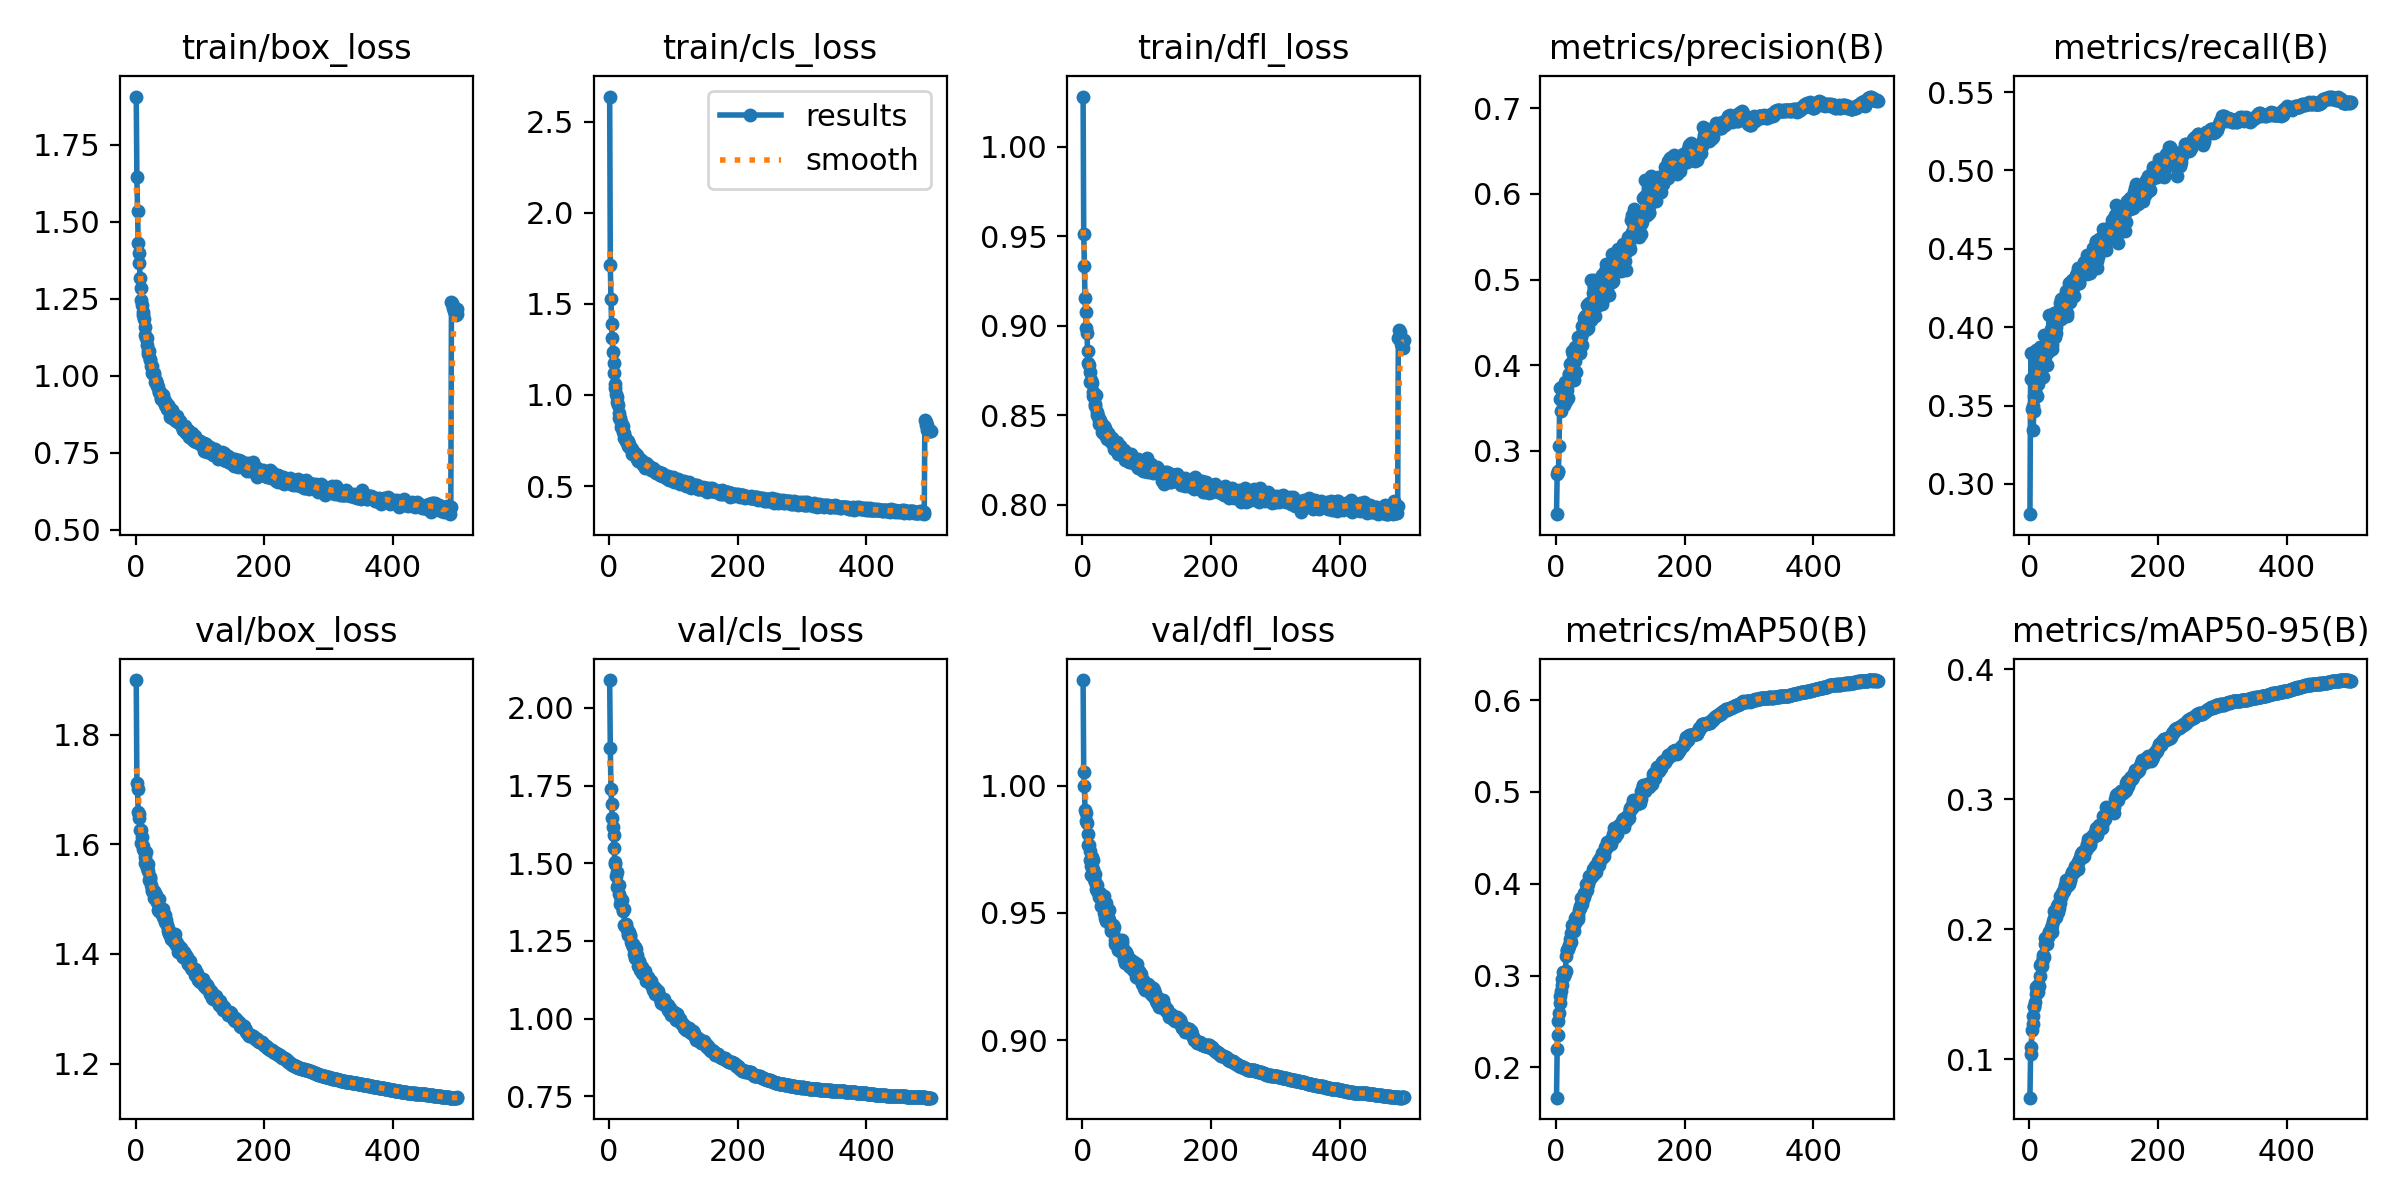
\includegraphics[width=0.8\textwidth]{v_3/results.png}
        \caption{Andamento funzioni di loss e metriche durante l'esecuzione di v8m12}
        \label{fig:v2-2}
    \end{figure}
    % - grafici recall e precision e performance e F1
    \begin{figure}[h]
        \centering
        \begin{subfigure}{.5\textwidth}
            \centering
            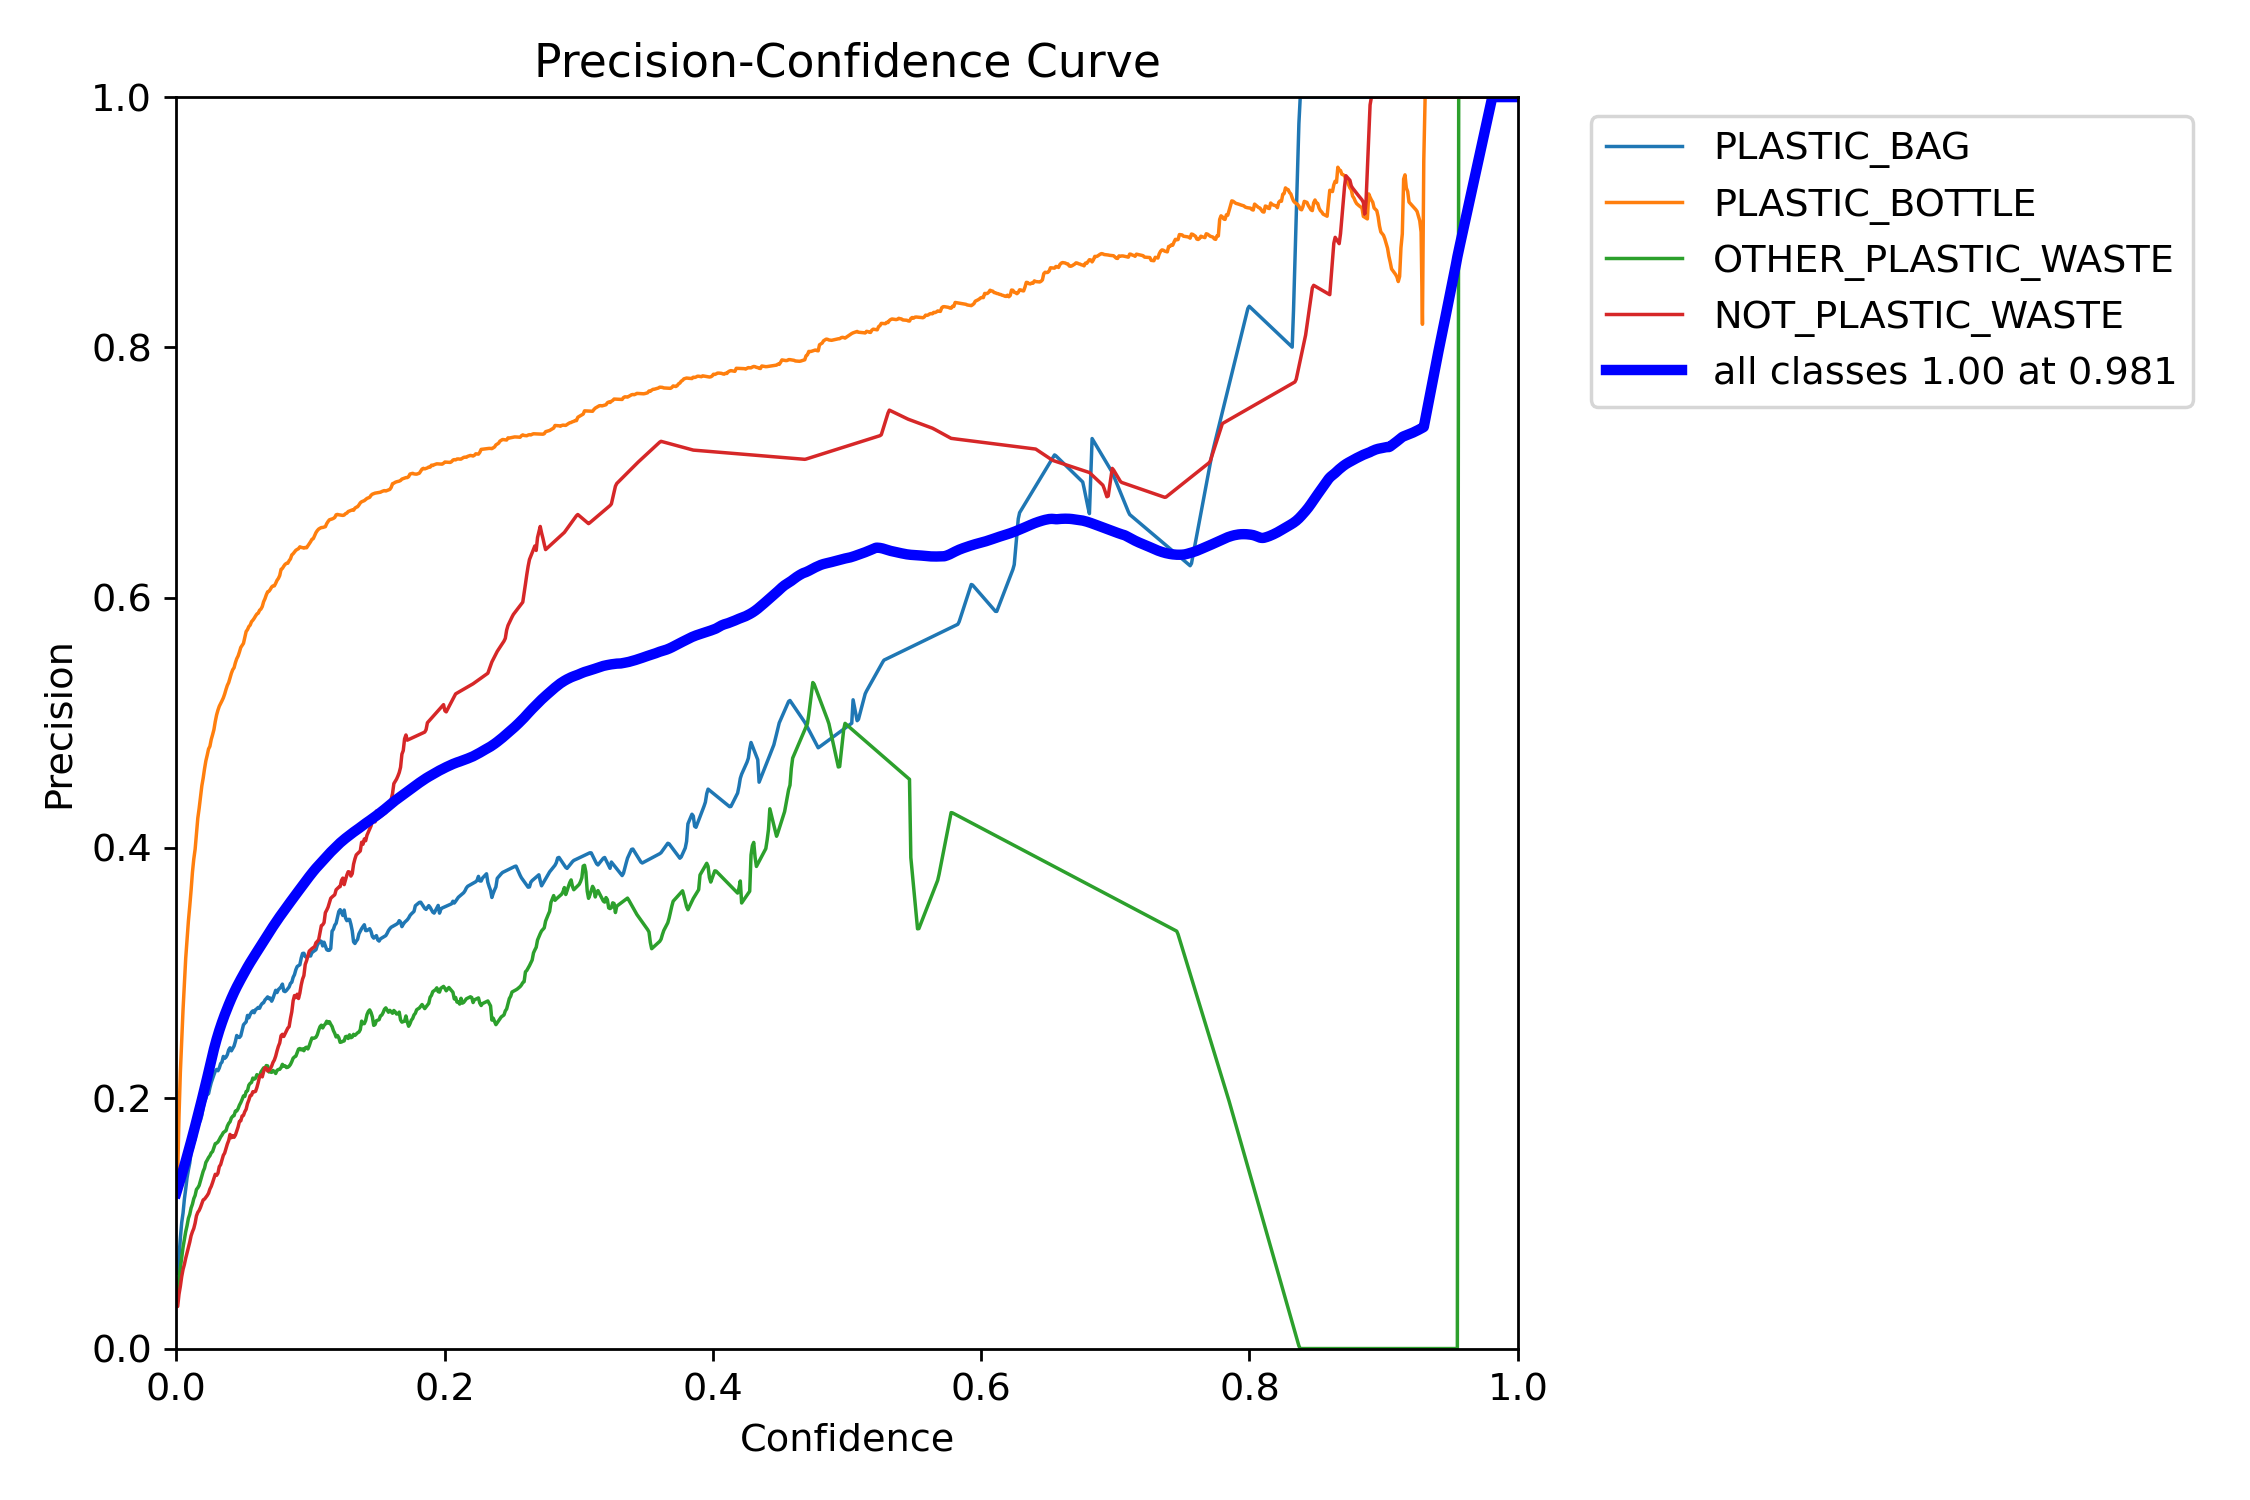
\includegraphics[width=.9\linewidth]{v_3/P_curve.png}
            
            \label{fig:v2-3.1}
          \end{subfigure}%
          \begin{subfigure}{.5\textwidth}
            \centering
            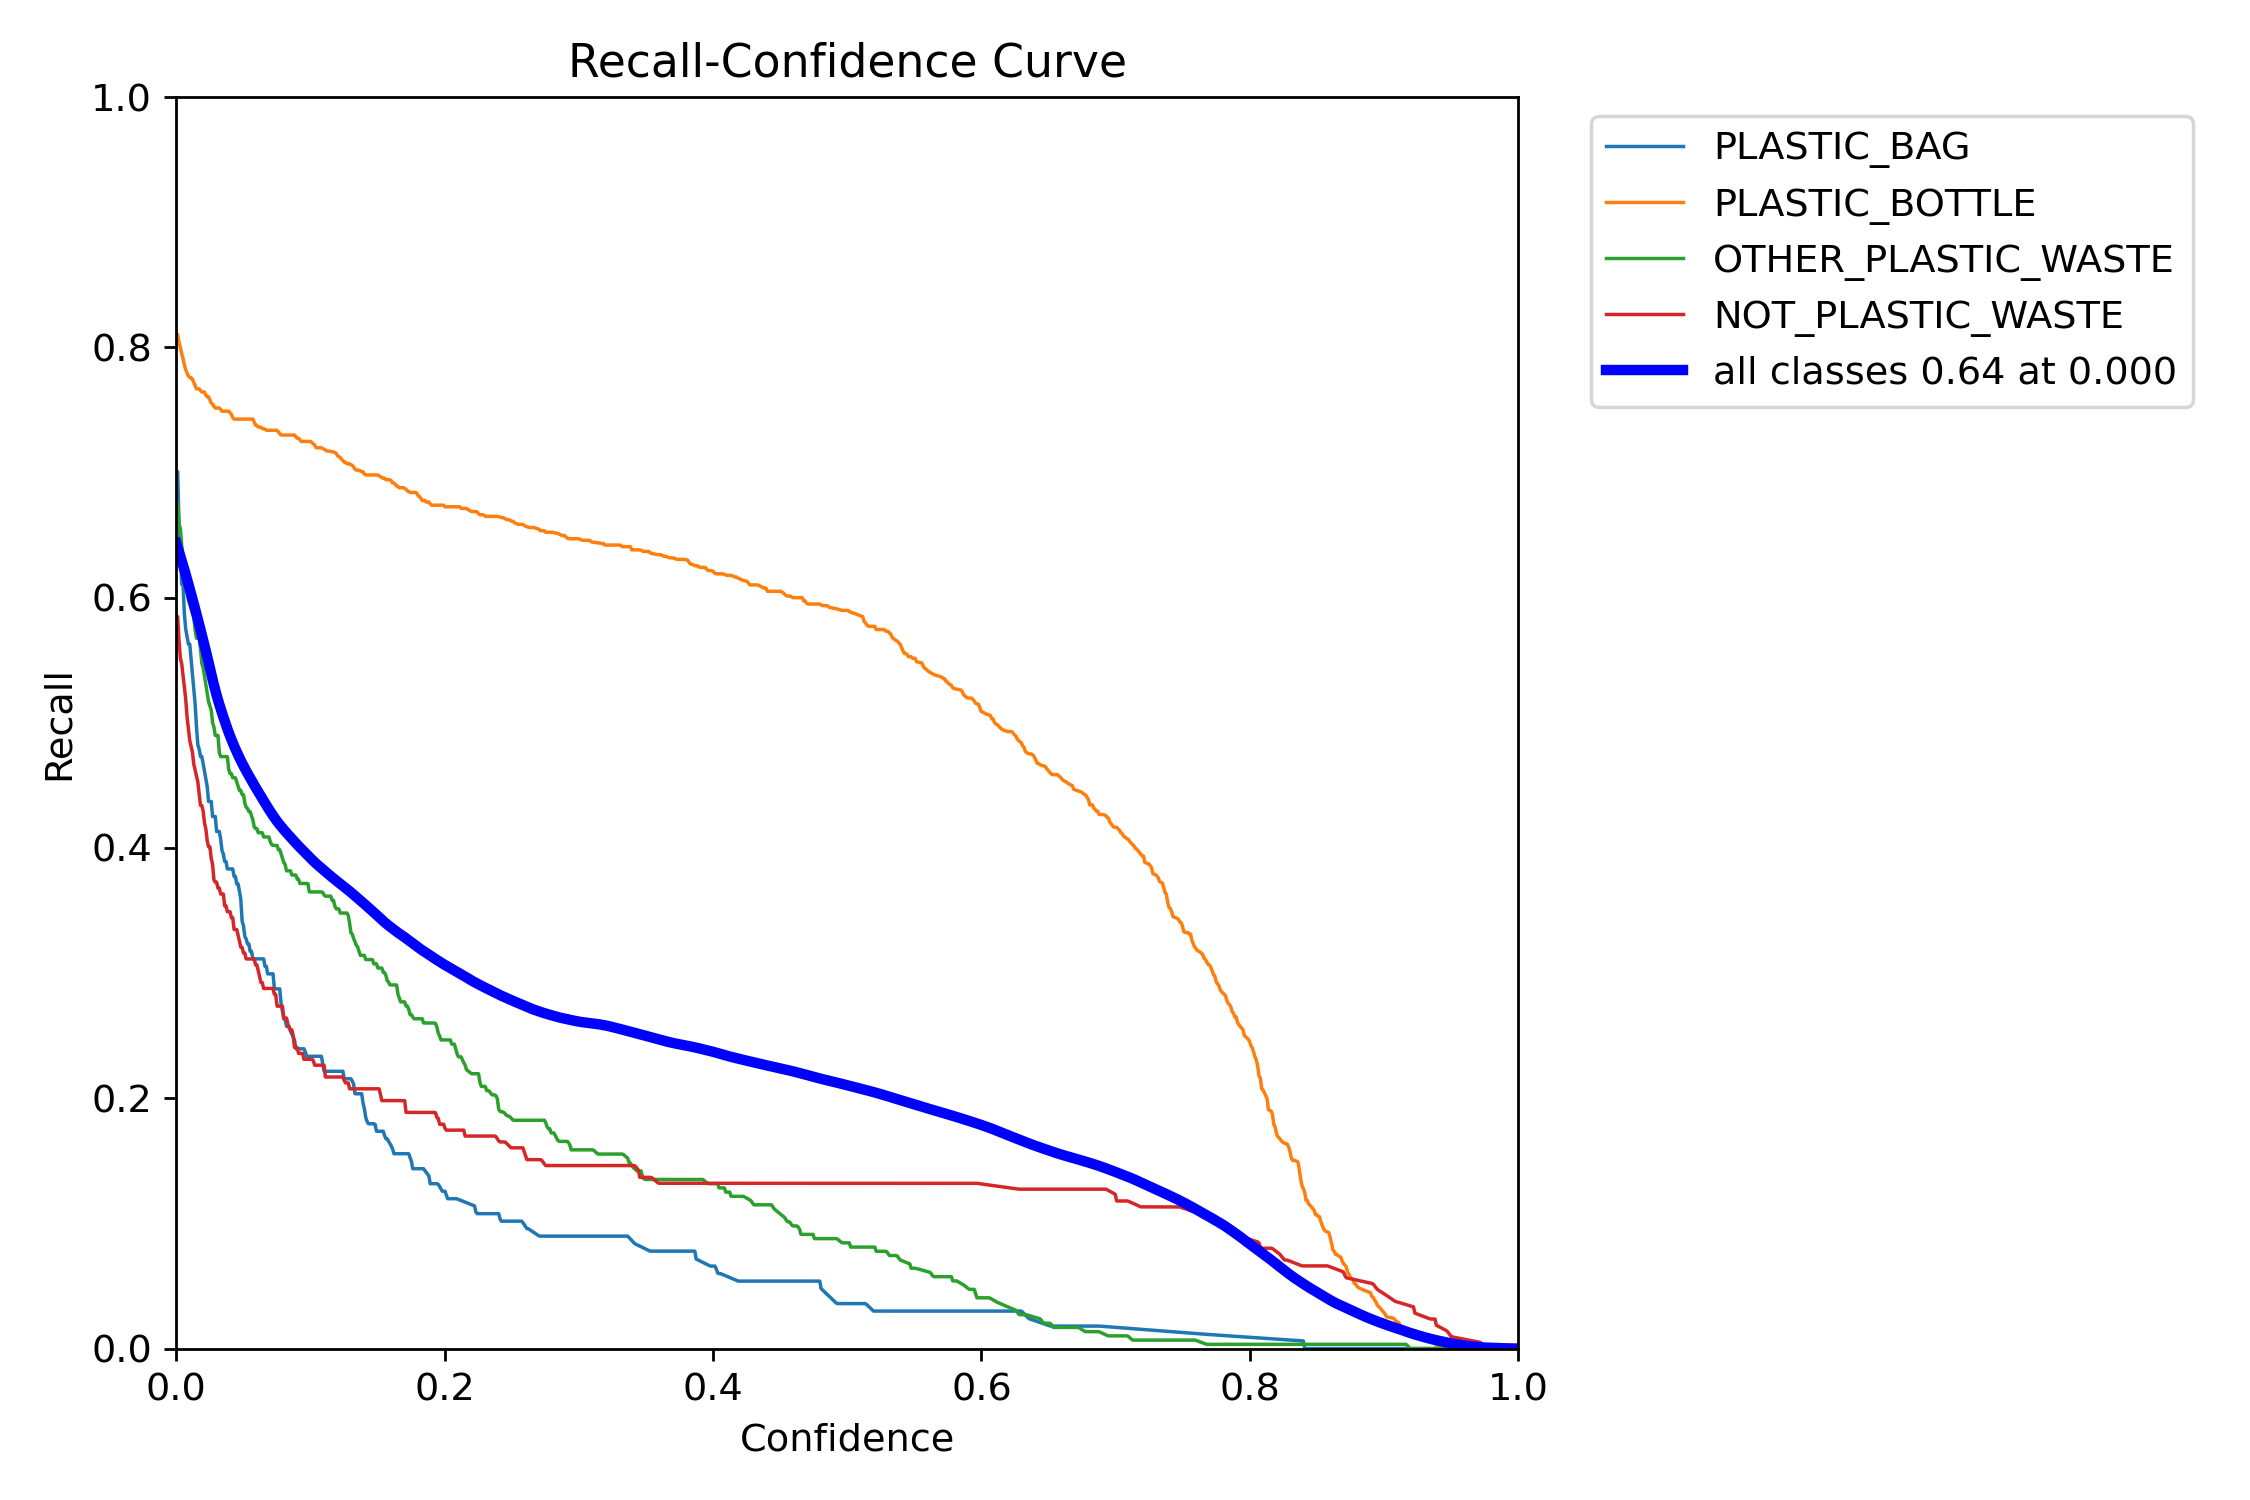
\includegraphics[width=.9\linewidth]{v_3/R_curve.png}
            
            \label{fig:v2-3.2}
          \end{subfigure}
          \vskip\baselineskip
        \begin{subfigure}{.5\textwidth}
          \centering
          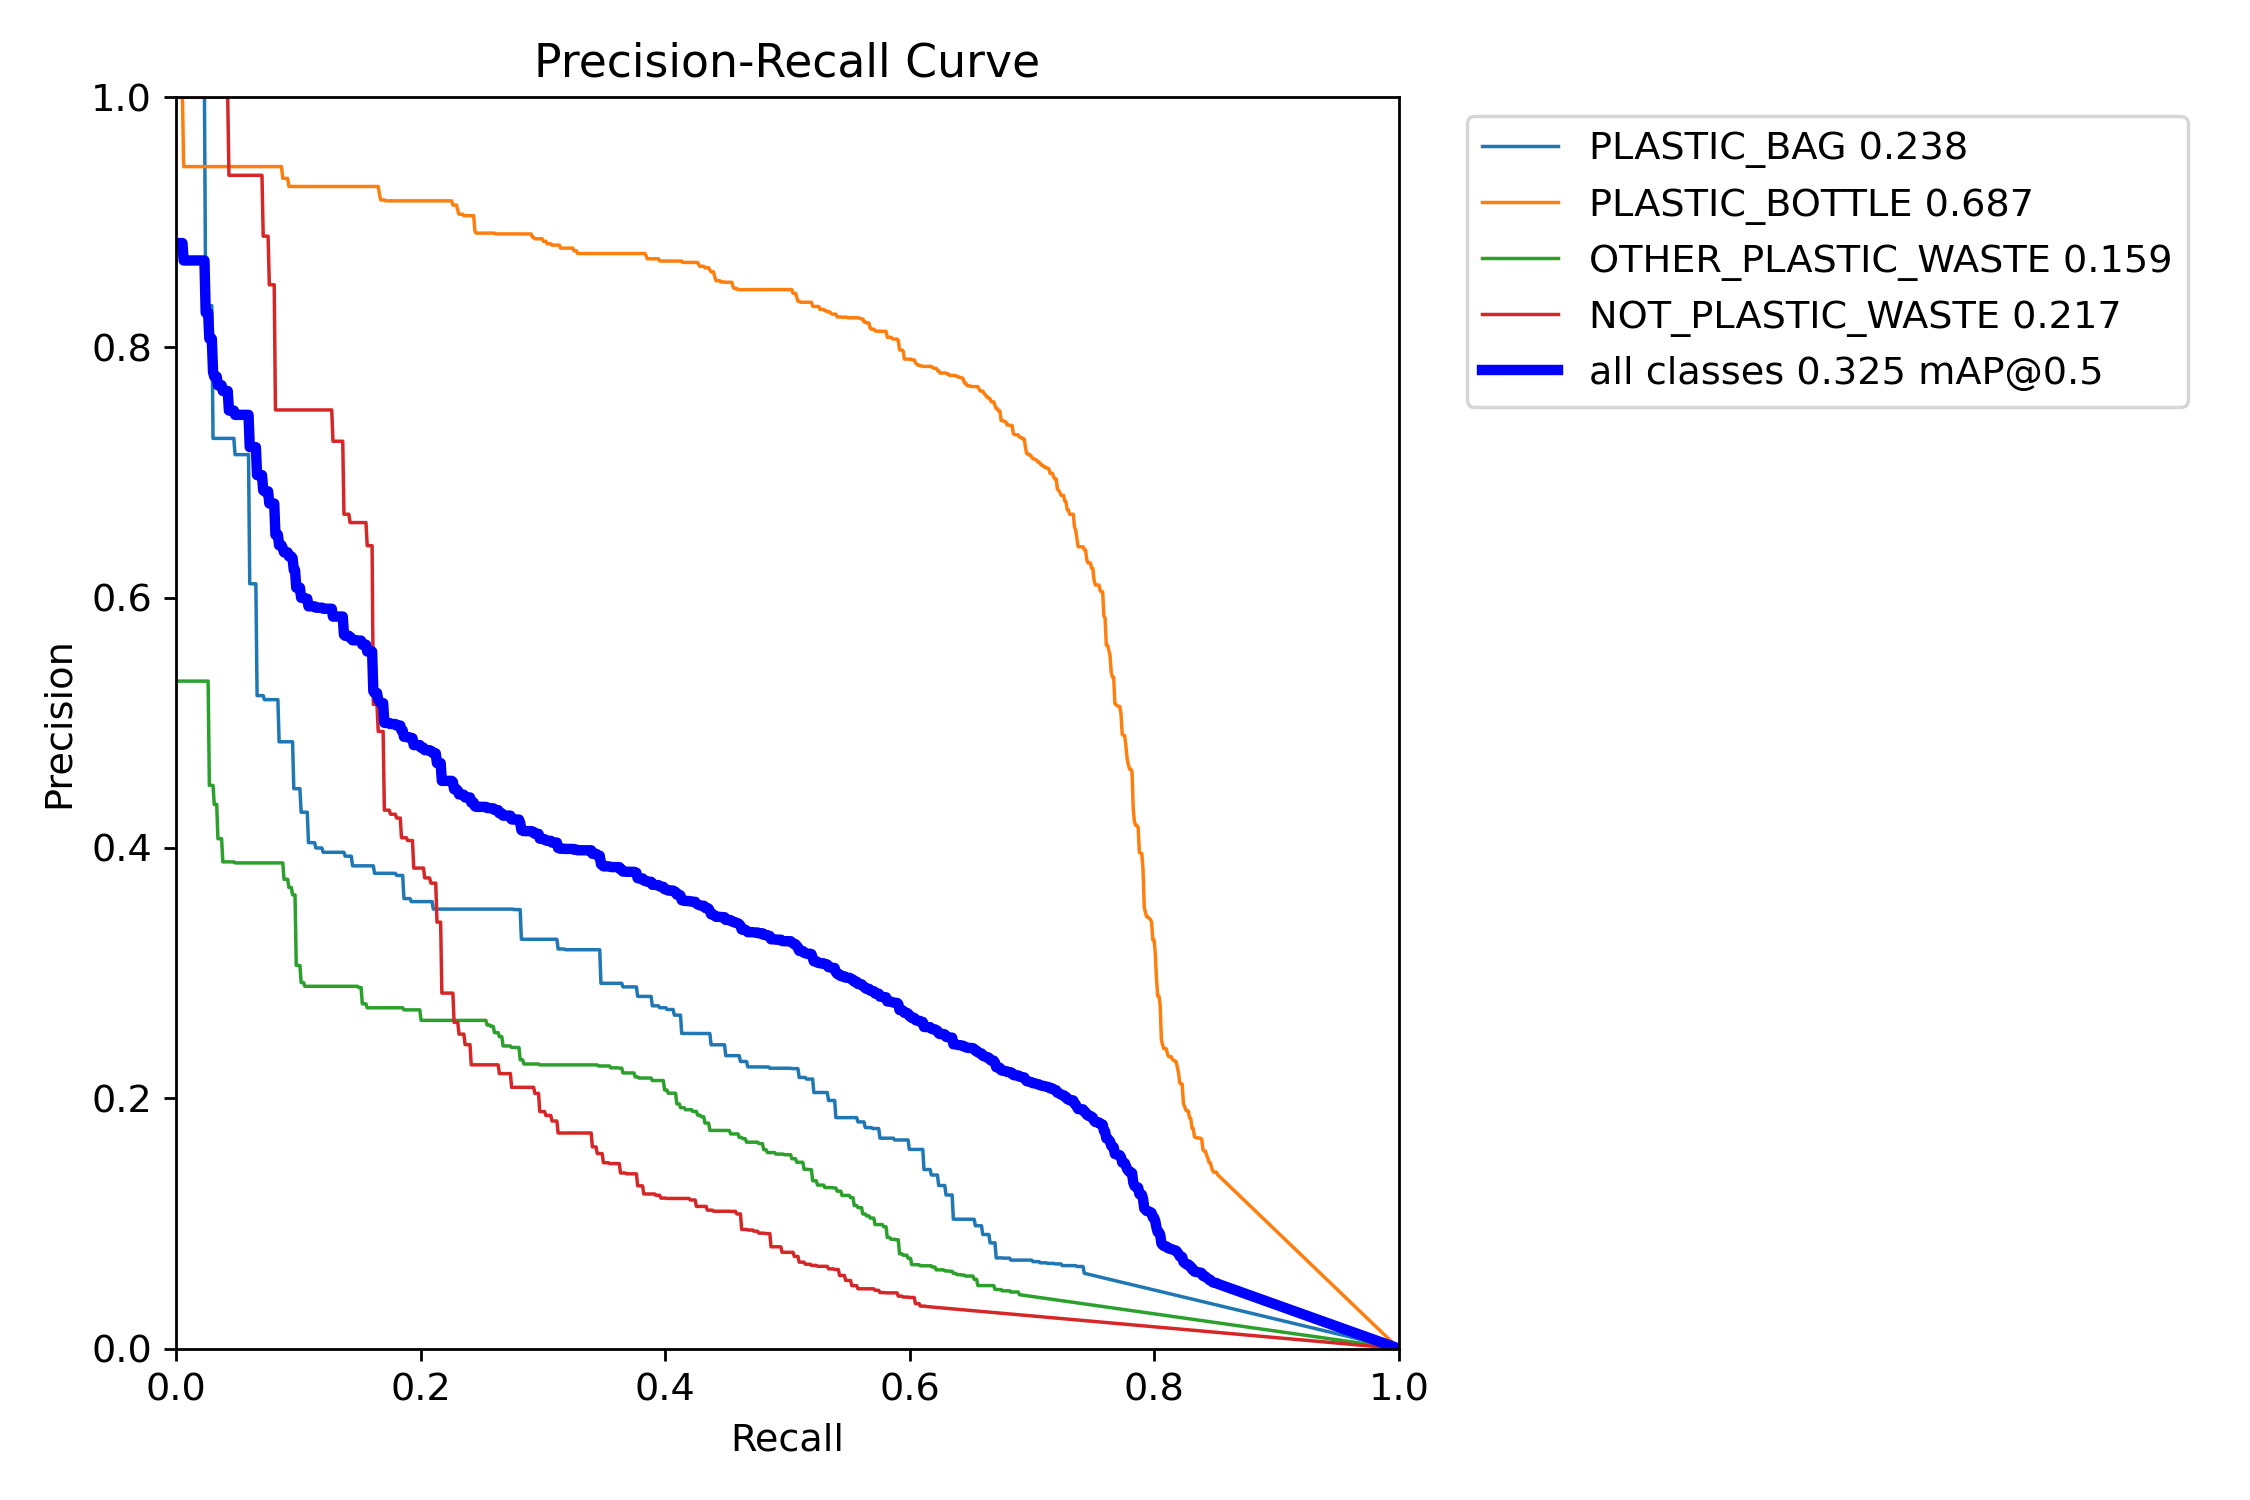
\includegraphics[width=.9\linewidth]{v_3/PR_curve.png}
          \label{fig:v2-3.3}
        \end{subfigure}
        \begin{subfigure}{.49\textwidth}
            \centering
            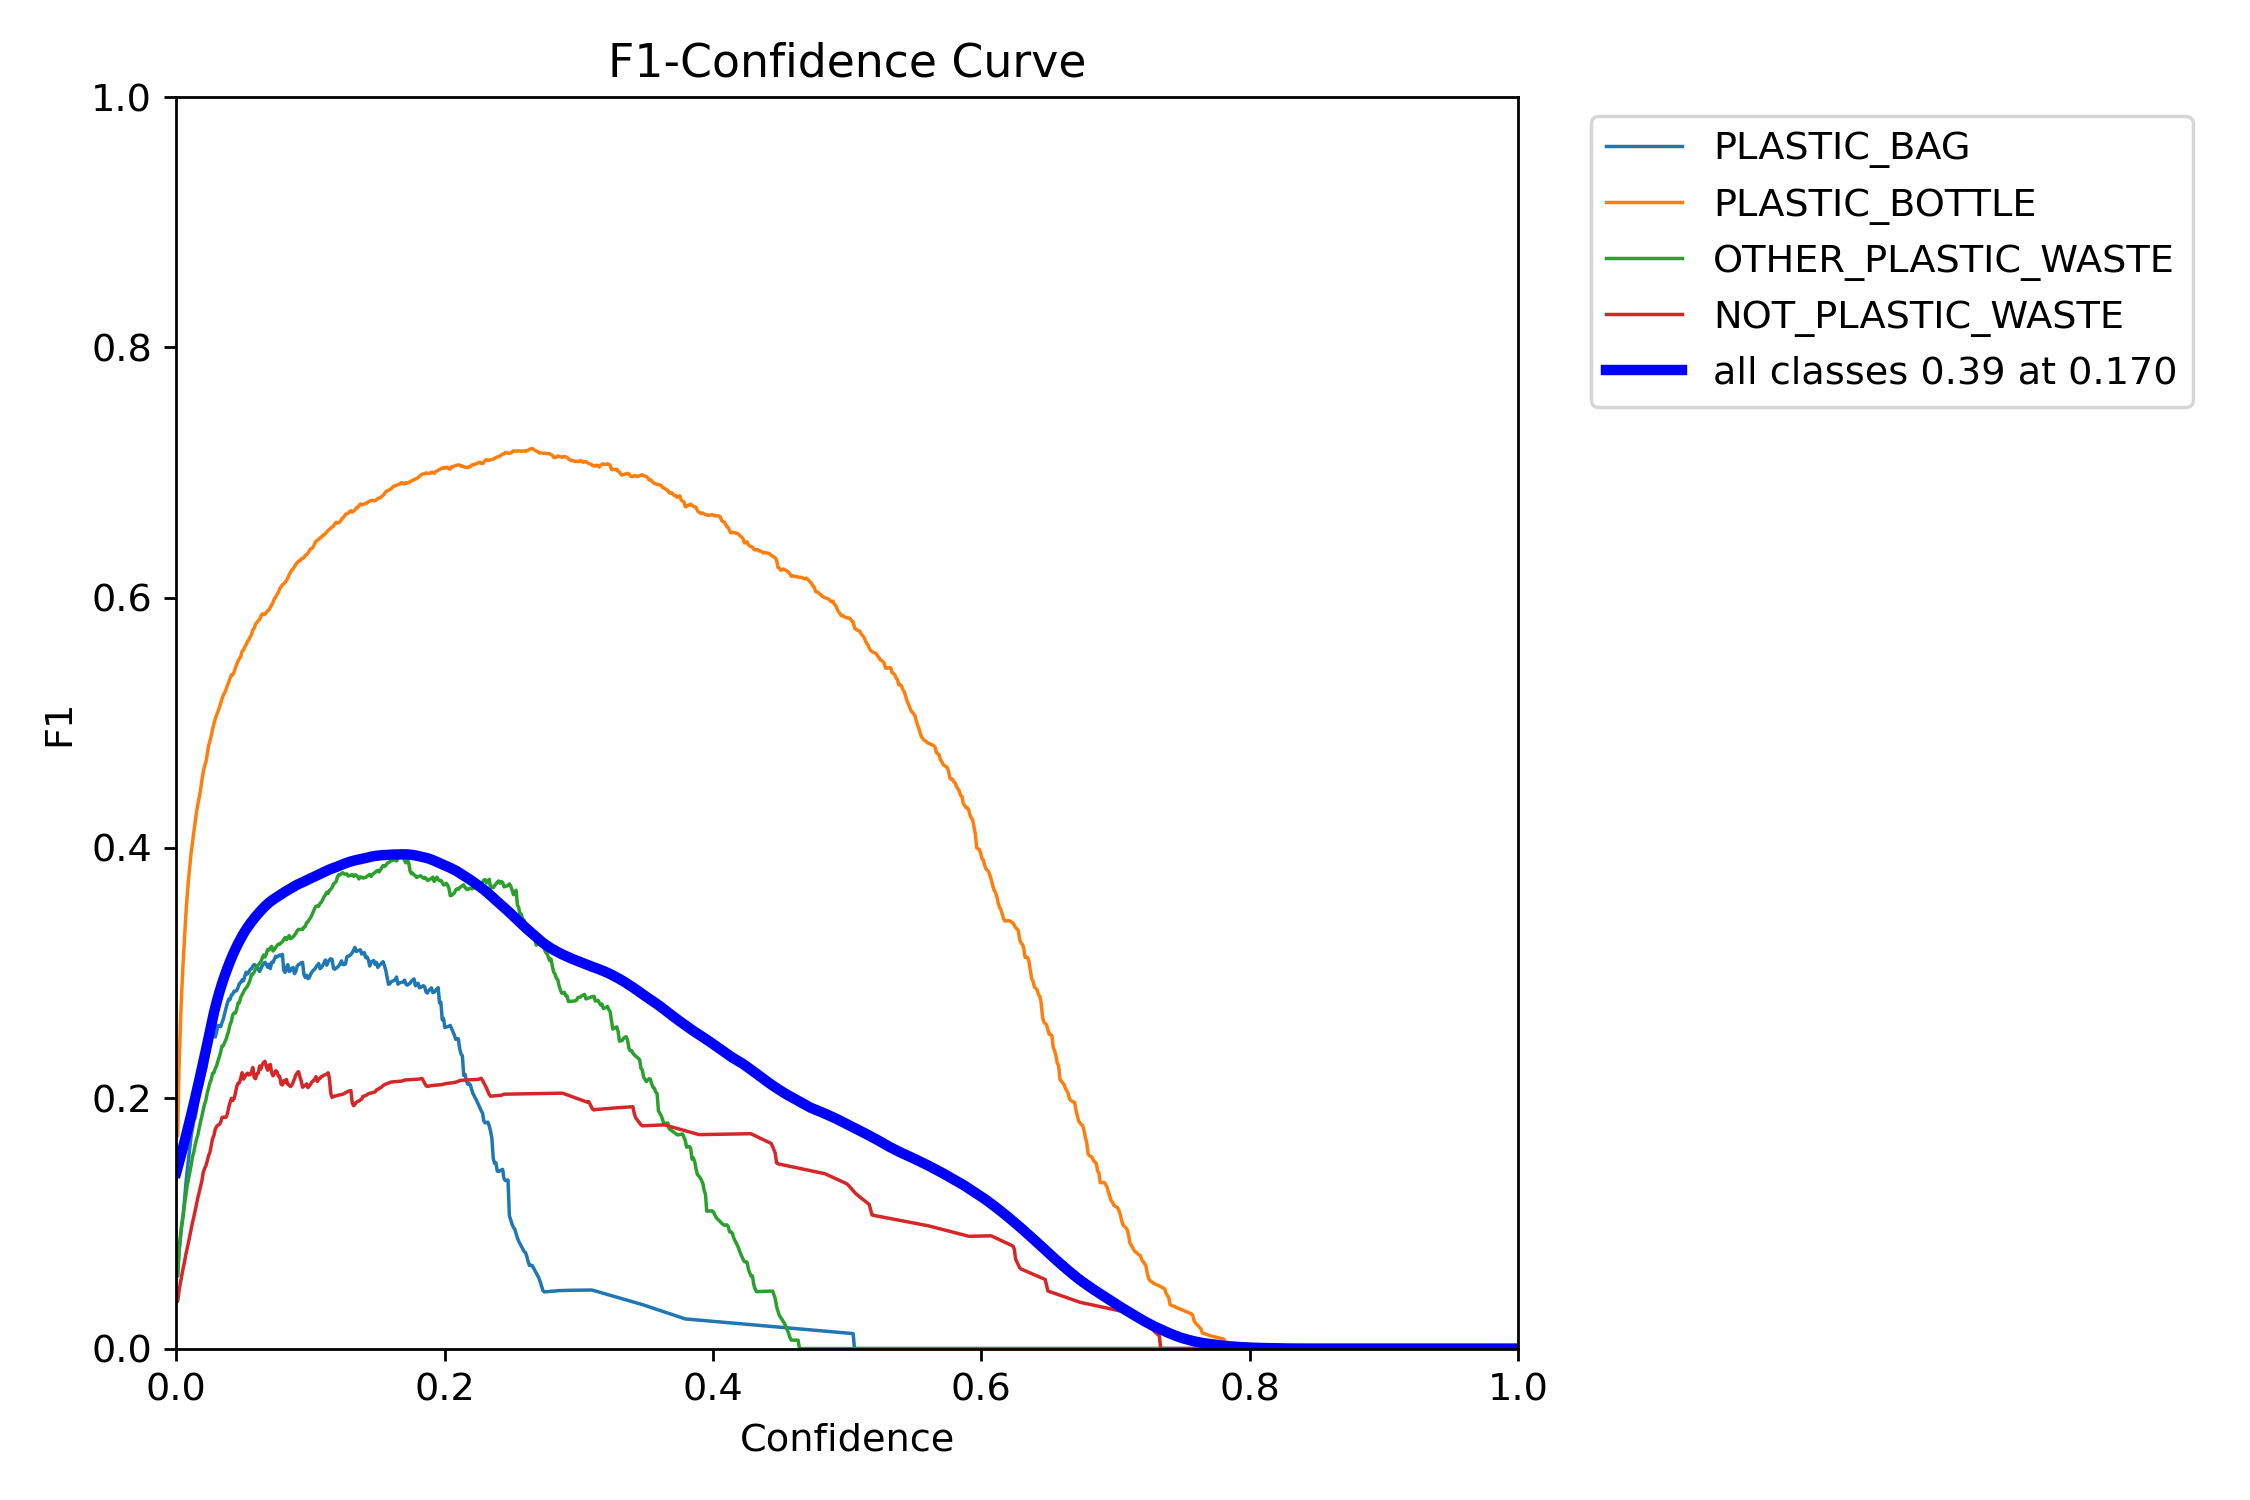
\includegraphics[width=.9\linewidth]{v_3/F1_curve.png}
            \label{fig:v2-3.4}
          \end{subfigure}

        \caption{Andamento funzioni di loss e metriche durante l'esecuzione di v8m12}
        \label{fig:v2-3}
    \end{figure}


    % - matrici di confusione
    \begin{figure}[h]
        \centering
        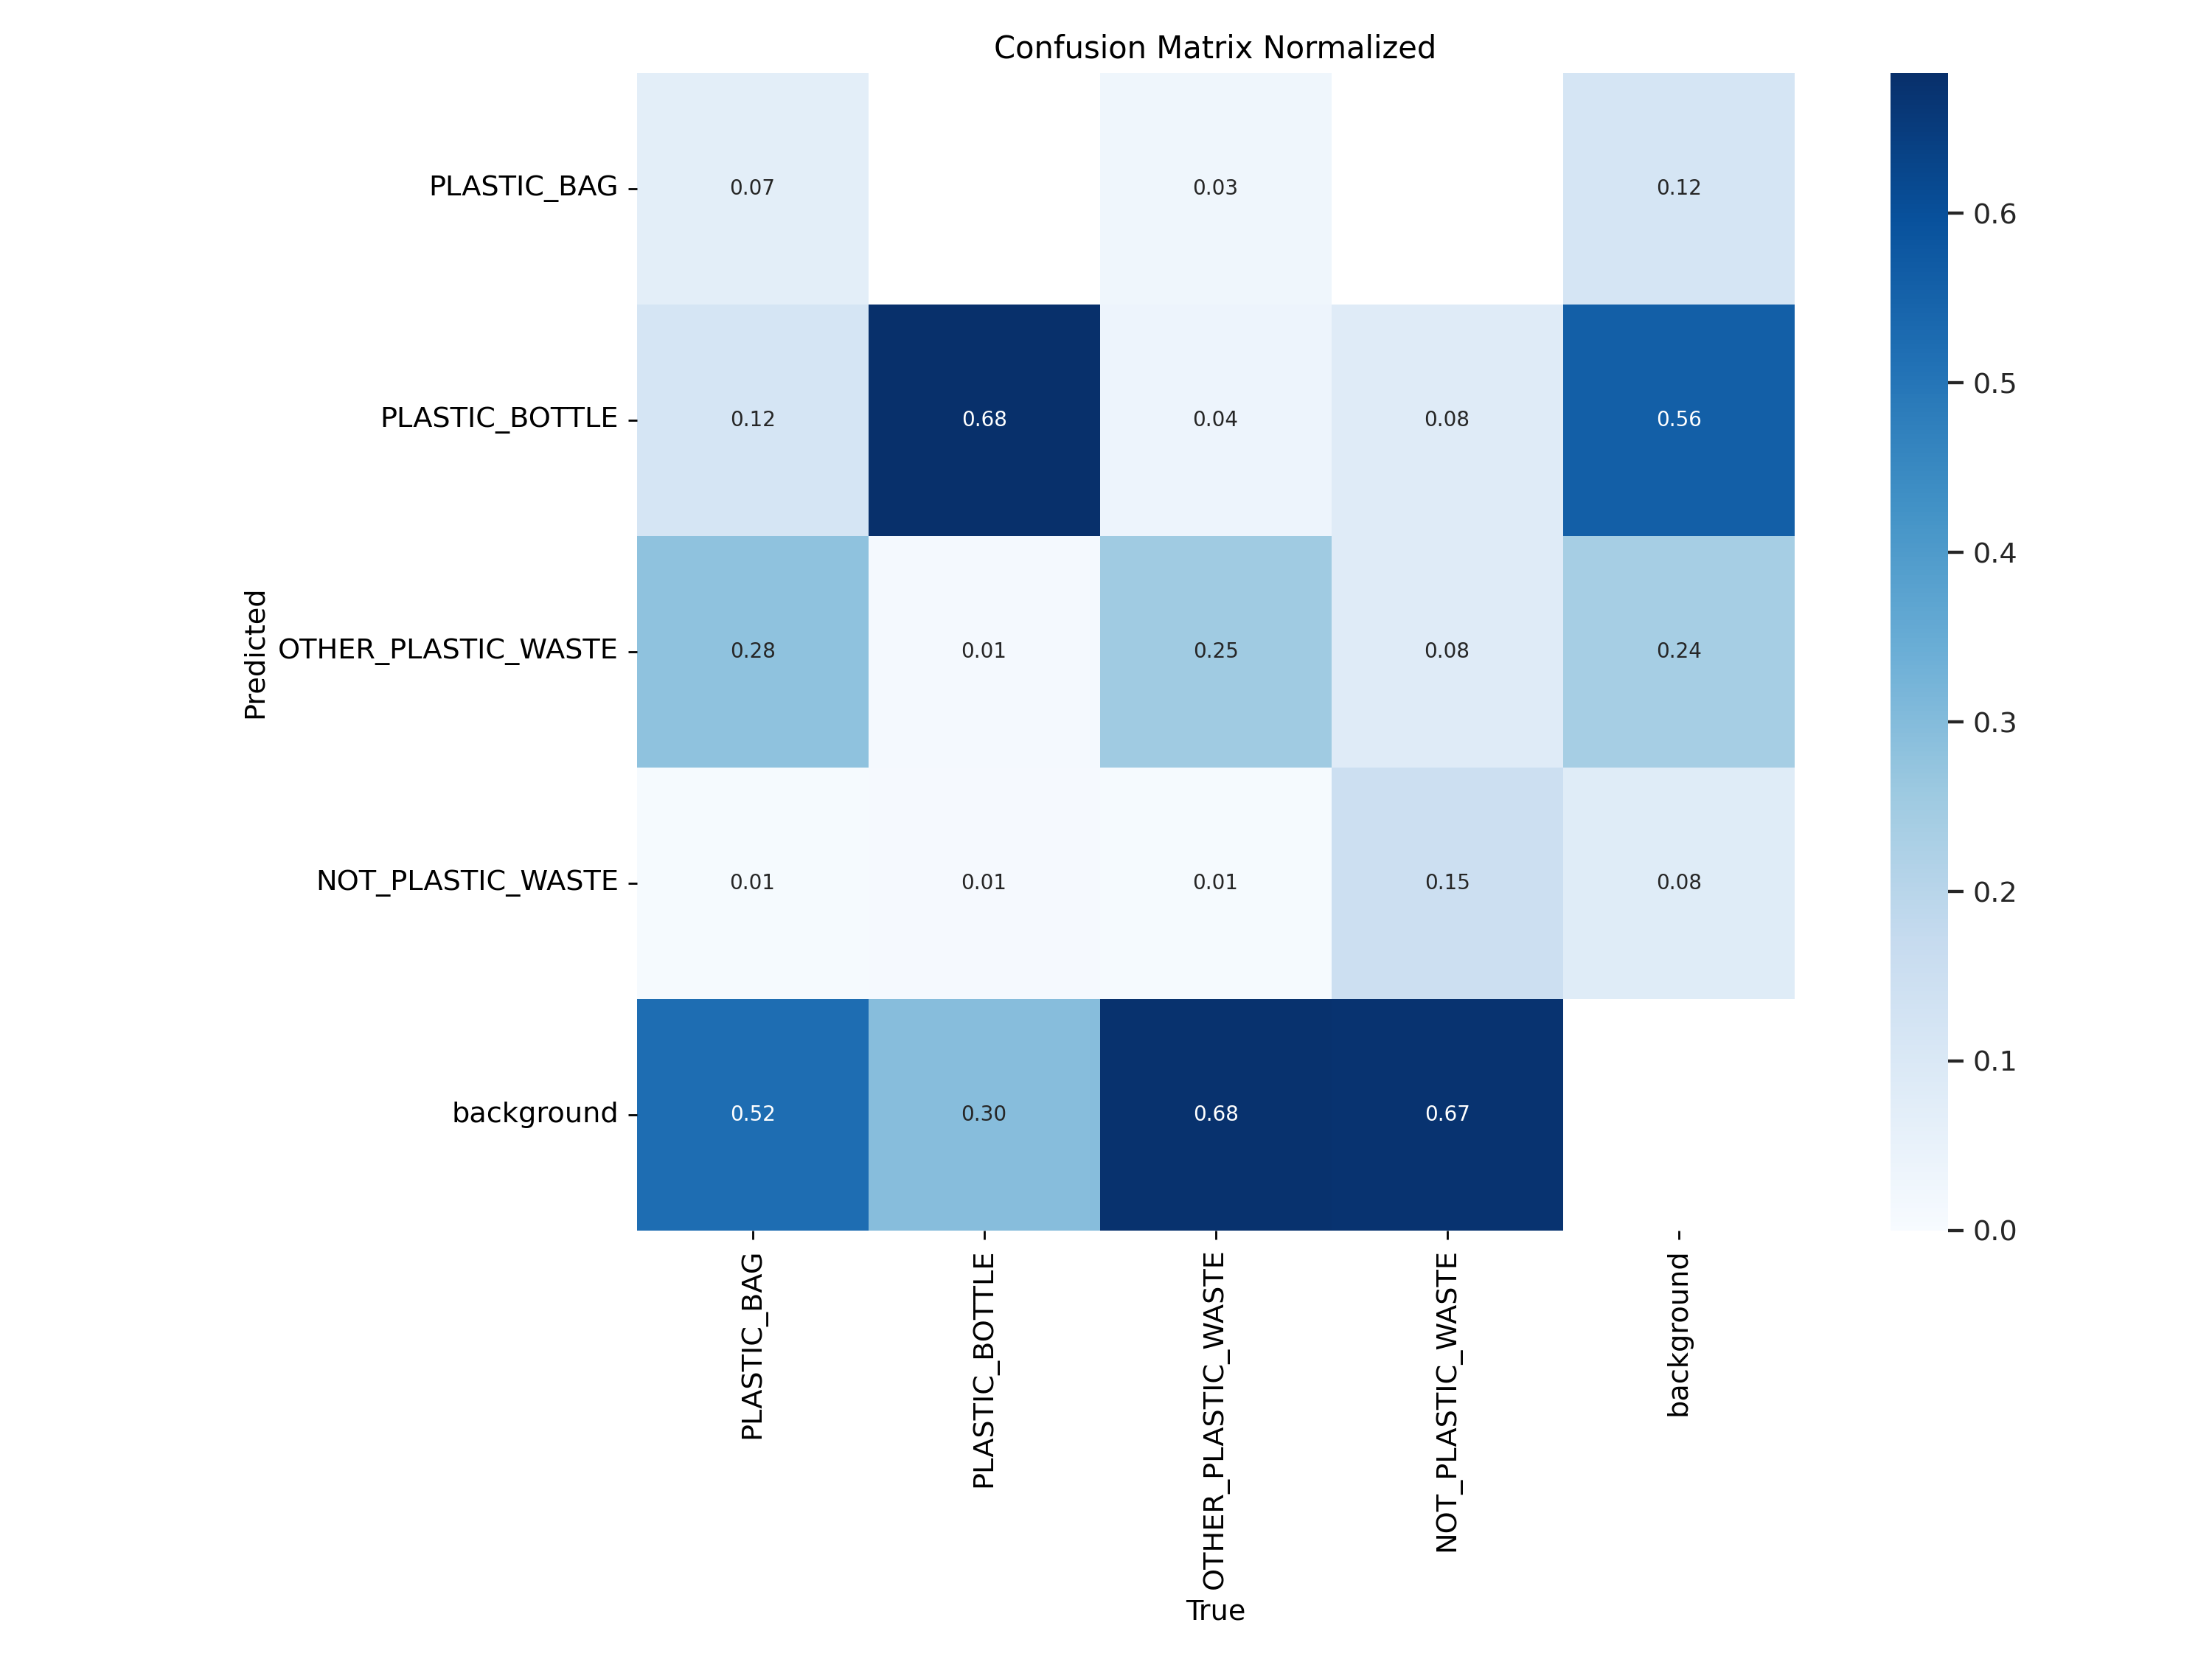
\includegraphics[width=0.8\textwidth]{v_3/confusion_matrix_normalized.png}
        \caption{Matrice di confusione normalizzata data dal modello medium-200-0}
        \label{fig:v2-4}
    \end{figure}
    % - tabella performance test set

primo modello